% Template adapted from https://github.com/jgm/pandoc-templates/blob/master/default.latex
% To be used with XeLaTex in memoiR
%%%%%%%%%%%%%%%%%%%%%%%%%%%%%%%%%%%%%%%%%%%%%%%%%%%%%%%%%%%%%%%%%%%%%%%%%%%%%%%%%%%%%%%%%

% Options for packages loaded elsewhere
\PassOptionsToPackage{unicode=true}{hyperref}
\PassOptionsToPackage{hyphens}{url}
\PassOptionsToPackage{dvipsnames,svgnames*,x11names*}{xcolor}
% Right to left support


\documentclass[
  12pt,
  american,
  a4paper,
  extrafontsizes,onecolumn,openright
  ]{memoir}

% Double (or whatever) spacing

% Math
\usepackage{amssymb, amsmath}
% mathspec: arbitrary math fonts
\usepackage{unicode-math}
\defaultfontfeatures{Scale=MatchLowercase}
\defaultfontfeatures[\rmfamily]{Ligatures=TeX,Scale=1}

% Fonts
\usepackage{lmodern}
\usepackage{fontspec}
% Main font
% Specific sanserif font
% Specific monotype font
% Specific math font
% Chinese, Japanese, Corean fonts

% Use upquote for straight quotes in verbatim environments
\usepackage{upquote}
% Use microtype
\usepackage[]{microtype}
\UseMicrotypeSet[protrusion]{basicmath} % disable protrusion for tt fonts

% Verbatim in note

% Color links
\usepackage{xcolor}

% Strikeout

% Necessary for code chunks
\usepackage{color}
\usepackage{fancyvrb}
\newcommand{\VerbBar}{|}
\newcommand{\VERB}{\Verb[commandchars=\\\{\}]}
\DefineVerbatimEnvironment{Highlighting}{Verbatim}{commandchars=\\\{\}}
% Add ',fontsize=\small' for more characters per line
\usepackage{framed}
\definecolor{shadecolor}{RGB}{248,248,248}
\newenvironment{Shaded}{\begin{snugshade}}{\end{snugshade}}
\newcommand{\AlertTok}[1]{\textcolor[rgb]{0.94,0.16,0.16}{#1}}
\newcommand{\AnnotationTok}[1]{\textcolor[rgb]{0.56,0.35,0.01}{\textbf{\textit{#1}}}}
\newcommand{\AttributeTok}[1]{\textcolor[rgb]{0.77,0.63,0.00}{#1}}
\newcommand{\BaseNTok}[1]{\textcolor[rgb]{0.00,0.00,0.81}{#1}}
\newcommand{\BuiltInTok}[1]{#1}
\newcommand{\CharTok}[1]{\textcolor[rgb]{0.31,0.60,0.02}{#1}}
\newcommand{\CommentTok}[1]{\textcolor[rgb]{0.56,0.35,0.01}{\textit{#1}}}
\newcommand{\CommentVarTok}[1]{\textcolor[rgb]{0.56,0.35,0.01}{\textbf{\textit{#1}}}}
\newcommand{\ConstantTok}[1]{\textcolor[rgb]{0.00,0.00,0.00}{#1}}
\newcommand{\ControlFlowTok}[1]{\textcolor[rgb]{0.13,0.29,0.53}{\textbf{#1}}}
\newcommand{\DataTypeTok}[1]{\textcolor[rgb]{0.13,0.29,0.53}{#1}}
\newcommand{\DecValTok}[1]{\textcolor[rgb]{0.00,0.00,0.81}{#1}}
\newcommand{\DocumentationTok}[1]{\textcolor[rgb]{0.56,0.35,0.01}{\textbf{\textit{#1}}}}
\newcommand{\ErrorTok}[1]{\textcolor[rgb]{0.64,0.00,0.00}{\textbf{#1}}}
\newcommand{\ExtensionTok}[1]{#1}
\newcommand{\FloatTok}[1]{\textcolor[rgb]{0.00,0.00,0.81}{#1}}
\newcommand{\FunctionTok}[1]{\textcolor[rgb]{0.00,0.00,0.00}{#1}}
\newcommand{\ImportTok}[1]{#1}
\newcommand{\InformationTok}[1]{\textcolor[rgb]{0.56,0.35,0.01}{\textbf{\textit{#1}}}}
\newcommand{\KeywordTok}[1]{\textcolor[rgb]{0.13,0.29,0.53}{\textbf{#1}}}
\newcommand{\NormalTok}[1]{#1}
\newcommand{\OperatorTok}[1]{\textcolor[rgb]{0.81,0.36,0.00}{\textbf{#1}}}
\newcommand{\OtherTok}[1]{\textcolor[rgb]{0.56,0.35,0.01}{#1}}
\newcommand{\PreprocessorTok}[1]{\textcolor[rgb]{0.56,0.35,0.01}{\textit{#1}}}
\newcommand{\RegionMarkerTok}[1]{#1}
\newcommand{\SpecialCharTok}[1]{\textcolor[rgb]{0.00,0.00,0.00}{#1}}
\newcommand{\SpecialStringTok}[1]{\textcolor[rgb]{0.31,0.60,0.02}{#1}}
\newcommand{\StringTok}[1]{\textcolor[rgb]{0.31,0.60,0.02}{#1}}
\newcommand{\VariableTok}[1]{\textcolor[rgb]{0.00,0.00,0.00}{#1}}
\newcommand{\VerbatimStringTok}[1]{\textcolor[rgb]{0.31,0.60,0.02}{#1}}
\newcommand{\WarningTok}[1]{\textcolor[rgb]{0.56,0.35,0.01}{\textbf{\textit{#1}}}}

% Listings package

% Tables
\usepackage{longtable,booktabs,tabu}
% Fix footnotes in tables (requires footnote package)
\IfFileExists{footnote.sty}{\usepackage{footnote}\makesavenoteenv{longtable}}{}

% Graphics
\usepackage{graphicx,grffile}
\graphicspath{{images/}}
\makeatletter
\def\maxwidth{\ifdim\Gin@nat@width>\linewidth\linewidth\else\Gin@nat@width\fi}
\def\maxheight{\ifdim\Gin@nat@height>\textheight\textheight\else\Gin@nat@height\fi}
\makeatother
% Scale images if necessary, so that they will not overflow the page
% margins by default, and it is still possible to overwrite the defaults
% using explicit options in \includegraphics[width, height, ...]{}
\setkeys{Gin}{width=\maxwidth,height=\maxheight,keepaspectratio}

% Prevent overfull lines
\setlength{\emergencystretch}{3em}  
\providecommand{\tightlist}{%
  \setlength{\itemsep}{0pt}\setlength{\parskip}{0pt}}

% Number sections for memoir (secnumdepth counter is ignored)
\setsecnumdepth{section}

% Set default figure placement to htbp
\makeatletter
\def\fps@figure{htbp}
\makeatother

% Spacing in lists
\usepackage{enumitem}

% Polyglossia
\usepackage{polyglossia}
\setmainlanguage{en-US}
\setotherlanguage{fr-FR}
\setotherlanguage{it}

% BibLaTeX
\usepackage[backend=biber,style=authoryear-ibid,isbn=false,backref=true,giveninits=true,uniquename=init,maxcitenames=2,maxbibnames=150,sorting=nyt,sortcites=false]{biblatex}
\addbibresource{references.bib}

% cslreferences environment required by pandoc > 2.7



%%%%%%%%%%%%%%%%%%%%%%%%%%%%%%%%%%%%%%%%%%%%%%%%%%%%%%%%%%
% memoiR format

% Chapter Summary environment 
\usepackage[tikz]{bclogo}
\newenvironment{Summary}
  {\begin{bclogo}[logo=\bctrombone, noborder=true, couleur=lightgray!50]{In a Nutshell}\parindent0pt}
  {\end{bclogo}}
% Syntax:
%
%```{block, type='Summary'}
% Deliver message here.
% ```

% scriptsize code 
\let\oldverbatim\verbatim
\def\verbatim{\oldverbatim\scriptsize}
% Applies to code blocks and R code results
% code chunk options size='scriptsize' applies only to R code and results
% if the code chunk sets a different size, \def\verbatim{...} is prioritary for code results 


% Layout
%%%%%%%%%%%%%%%%%%%%%%%%%%%%%%%%%%%%%%%%%%%%%%%%%%%%%%%%%%

% Based on memoir, style companion
\newcommand{\MemoirChapStyle}{daleif1}
\newcommand{\MemoirPageStyle}{Ruled}

% Space between paragraphs
\usepackage{parskip}
  \abnormalparskip{3pt}

% Adjust margin paragraphs vertical position
\usepackage{marginfix}


% Margins
%%%%%%%%%%%%%%%%%%%%%%%%%%%%%%%%%%%%%%%

% allow use of '-',+','/' ans '*' to make simple length computation
\usepackage{calc}

% Full-width figures utilities
\newlength\widthw % full width
\newlength{\rf}
\newcommand*{\definesHSpace}{
  \strictpagecheck % slower but efficient detection of odd/even pages
  \checkoddpage
  \ifoddpage
  \setlength{\rf}{0mm}
  \else
  \setlength{\rf}{\marginparsep+\marginparwidth}
  \fi
}

\makeatletter
% 1" margins for the front matter.
\newcommand*{\SmallMargins}{
  \setlrmarginsandblock{1.5in}{1.5in}{*}
  \setmarginnotes{0.1in}{0.1in}{0.1in}
 \setulmarginsandblock{1.5in}{1in}{*}
  \checkandfixthelayout
  \ch@ngetext
  \clearpage
  \setlength{\widthw}{\textwidth+\marginparsep+\marginparwidth}
  \footnotesatfoot
  \chapterstyle{\MemoirChapStyle}  % Chapter and page styles must be recalled
  \pagestyle{\MemoirPageStyle}
}

% 3" outer margin for the main matter
\newcommand{\LargeMargins}{\SmallMargins}
\makeatother

% Figure captions and footnotes in outer margins


% Main title page with filigrane
%%%%%%%%%%%%%%%%%%%%%%%%%%%%%%%%%%%%%%%%%%%%%%%%%%%%%%%%%%

% Text blocks
\usepackage[absolute,overlay]{textpos}
  \setlength{\TPHorizModule}{1mm}
  \setlength{\TPVertModule}{1mm}

\newcommand{\MainTitlePage}[2]{
  \SmallMargins % Margins
  \pagestyle{empty} % No header/footer
  \textblockorigin{\stockwidth-\paperwidth-\trimedge}{\trimtop} % recto
  \begin{textblock*}{2mm}(\spinemargin/2,\uppermargin/2)
    \rule{1pt}{\paperheight-\uppermargin}
  \end{textblock*}
  \begin{textblock*}{\paperwidth*2/3}(\paperwidth/5, \paperheight/5)
    \flushright
    \begin{Spacing}{3}
      {\fontfamily{qtm}\selectfont\fontsize{45}{45}\selectfont\textsc{\thetitle}}
    \end{Spacing}
  \end{textblock*}
    \begin{textblock*}{\paperwidth*2/3}(\paperwidth/5, \paperheight/2)
    \flushright
    {\fontfamily{qtm}\huge\theauthor}
  \end{textblock*}
    \begin{textblock*}{\paperwidth*2/3}[0, 1](\spinemargin, \uppermargin+\textheight)
    \normalfont\thedate
  \end{textblock*}
  ~\\ % Print a character or the page will not exist
  \newpage
  \textblockorigin{\trimedge}{\trimtop} % verso
  \begin{textblock*}{\textwidth}(\paperwidth-\spinemargin-\textwidth, \uppermargin)
    #1
  \end{textblock*}
  \begin{textblock*}{\textwidth}[0,1](\paperwidth-\spinemargin-\textwidth, \uppermargin+\textheight+\footskip)
    \centering
    
\includegraphics[width=\paperwidth/4]{logo}\\ \bigskip
    #2
  \end{textblock*}
  ~\\ % Print a character or the page will not exist
  \newpage
}

% Clear page and open an even one (\clearpage opens an odd one)
\newcommand{\evenpage}{
  \clearpage
  \strictpagecheck % slower but efficient detection of odd/even pages
  \checkoddpage
  \ifoddpage
    \thispagestyle{empty}
    ~\\ % Print a character or the page will not exist
    \newpage
  \else
    % do nothing
  \fi
}


%% PDF title page to insert
%%%%%%%%%%%%%%%%%%%%%%%%%%%%%%%%%%%%%%%%%%%%%%%%%%%%%%%%%%

\usepackage{pdfpages}


%% Bibliography
%%%%%%%%%%%%%%%%%%%%%%%%%%%%%%%%%%%%%%%%%%%%%%%%%%%%%%%%%%

\usepackage[strict,autostyle]{csquotes}
% Repeated citation as author-year-title instead of author-title (modification of footcite:note in verbose-inote.cbx)

%% Table of Contents
%%%%%%%%%%%%%%%%%%%%%%%%%%%%%%%%%%%%%%%%%%%%%%%%%%%%%%%%%%

% fix the typesetting of the part number
\renewcommand\partnumberlinebox[2]{#2\ ---\ }


% Fonts
%%%%%%%%%%%%%%%%%%%%%%%%%%%%%%%%%%%%%%%%%%%%%%%%%%%%%%%%%%


% Hyperref comes last
%%%%%%%%%%%%%%%%%%%%%%%%%%%%%%%%%%%%%%%%%%%%%%%%%%%%%%%%%%

\usepackage{hyperref}
\hypersetup{
  pdftitle={Title of the Memoir},
  pdfauthor={Authors' names},
  colorlinks=true,
  linkcolor=Maroon,
  citecolor=Blue,
  urlcolor=Blue,
  breaklinks=true}

% Don't use monospace font for urls
\urlstyle{same}


% Title, author, date from YAML to LaTeX
%%%%%%%%%%%%%%%%%%%%%%%%%%%%%%%%%%%%%%%%%%%%%%%%%%%%%%%%%%

\title{Title of the Memoir}

\author{Authors' names}

\date{2022-06-03}


% Include headers (preamble.tex) here
%%%%%%%%%%%%%%%%%%%%%%%%%%%%%%%%%%%%%%%%%%%%%%%%%%%%%%%%%%
% Add LaTeX code into the preamble of the document here
\hyphenation{bio-di-ver-si-ty sap-lings}


%%%%%%%%%%%%%%%%%%%%%%%%%%%%%%%%%%%%%%%%%%%%%%%%%%%%%%%%%%%%%%%%%%%%%%%%%
% memoiR dalef3 chapter style 
% https://ctan.crest.fr/tex-archive/info/latex-samples/MemoirChapStyles/MemoirChapStyles.pdf
\usepackage{soul}
\definecolor{nicered}{rgb}{.647,.129,.149}
\makeatletter
\newlength\dlf@normtxtw
\setlength\dlf@normtxtw{\textwidth}
\def\myhelvetfont{\def\sfdefault{mdput}}
\newsavebox{\feline@chapter}
\newcommand\feline@chapter@marker[1][4cm]{%
  \sbox\feline@chapter{%
    \resizebox{!}{#1}{\fboxsep=1pt%
	  \colorbox{nicered}{\color{white}\bfseries\sffamily\thechapter}%
	}}%
  \rotatebox{90}{%
    \resizebox{%
	  \heightof{\usebox{\feline@chapter}}+\depthof{\usebox{\feline@chapter}}}%
	{!}{\scshape\so\@chapapp}}\quad%
  \raisebox{\depthof{\usebox{\feline@chapter}}}{\usebox{\feline@chapter}}%
 }
\newcommand\feline@chm[1][4cm]{%
  \sbox\feline@chapter{\feline@chapter@marker[#1]}%
  \makebox[0pt][l]{% aka \rlap
    \makebox[1cm][r]{\usebox\feline@chapter}%
  }}
\makechapterstyle{daleif1}{
  \renewcommand\chapnamefont{\normalfont\Large\scshape\raggedleft\so}
  \renewcommand\chaptitlefont{\normalfont\huge\bfseries\scshape\color{nicered}}
  \renewcommand\chapternamenum{}
  \renewcommand\printchaptername{}
  \renewcommand\printchapternum{\null\hfill\feline@chm[2.5cm]\par}
  \renewcommand\afterchapternum{\par\vskip\midchapskip}
  \renewcommand\printchaptertitle[1]{\chaptitlefont\raggedleft ##1\par}
}
\makeatother


% End of preamble
%%%%%%%%%%%%%%%%%%%%%%%%%%%%%%%%%%%%%%%%%%%%%%%%%%%%%%%%%%


\begin{document}
\frontmatter

% Title page
%%%%%%%%%%%%%%%%%%%%%%%%%%%%%%%%%%%%%%%%%%%%%%%%%%%%%%%%%%


\includepdf[pages=1]{images/cover.pdf}
\cleardoublepage

\MainTitlePage{This document is reproducible thanks to:

\begin{itemize}
  \item \LaTeX and its class memoir (\url{http://www.ctan.org/pkg/memoir}).
  \item R (\url{http://www.r-project.org/}) and RStudio (\url{http://www.rstudio.com/})
  \item bookdown (\url{http://bookdown.org/}) and memoiR (\url{https://ericmarcon.github.io/memoiR/})
\end{itemize}}{Name of the owner of the logo

\url{http://www.company.com}

An explanatory sentence.
Leave an empty line for line breaks.}


% Before Body
%%%%%%%%%%%%%%%%%%%%%%%%%%%%%%%%%%%%%%%%%%%%%%%%%%%%%%%%%%





% Contents
%%%%%%%%%%%%%%%%%%%%%%%%%%%%%%%%%%%%%%%%%%%%%%%%%%%%%%%%%%

\LargeMargins
{
\hypersetup{linkcolor=}
\setcounter{tocdepth}{2}
\tableofcontents
}


% Body
%%%%%%%%%%%%%%%%%%%%%%%%%%%%%%%%%%%%%%%%%%%%%%%%%%%%%%%%%%

\LargeMargins
\hypertarget{introduction}{%
\chapter*{Introduction}\label{introduction}}
\addcontentsline{toc}{chapter}{Introduction}

This document allows you to create a book in PDF format (and ePub format) at the same time as an HTML version to be published on the web.
The syntax is that of \textbf{Markdown} with some extensions.

The \textbf{bookdown} package must be installed from CRAN or GitHub:

\scriptsize

\begin{Shaded}
\begin{Highlighting}[]
\FunctionTok{install.packages}\NormalTok{(}\StringTok{"bookdown"}\NormalTok{)}
\CommentTok{\# or the development version}
\CommentTok{\# devtools::install\_github(\textquotesingle{}rstudio/bookdown\textquotesingle{})}
\end{Highlighting}
\end{Shaded}

\normalsize

The book is organized in chapters.
Each chapter is an Rmd file, whose name normally begins with its number (e.g.~\texttt{01-intro.Rmd}).
All Rmd files in the project folder are actually treated as chapters, sorted by filename.
The index.Rmd file is special: it contains the document header and the first chapter.

This first chapter is placed in the foreword of the printed book: it should not be numbered (hence the \texttt{\{-\}} code next to the title) in the HTML version.
It must end with the LaTeX command \texttt{\textbackslash{}mainmatter} which marks the beginning of the body of the book.

The outline levels start with \texttt{\#} for chapters (only one per file), \texttt{\#\#} for sections, etc.

Compilation in PDF format is done by XeLaTeX, which must be installed.

While writing, it is strongly advised to create only the HTML file, which is much faster than a LaTeX compilation.
Each chapter can be viewed very quickly by clicking on the \emph{Knit} button above the source window.
The entire book is created by clicking on the \emph{Build Book} button in the RStudio \emph{Build} window.
The button's drop-down list allows you to create all documents or limit yourself to one format.

\mainmatter

\hypertarget{getting_started}{%
\chapter{Getting Started}\label{getting_started}}

\emph{RStudio} in version higher than 1 must be used.
The \textbf{bookdown} package must be installed.

For the creation of the PDF file, an installation of LaTeX is necessary.
Under Windows, use \href{https://miktex.org/download}{MikTex}.
The automatic download of missing packages (under Windows: MiKTeX settings, \emph{Install missing packages=Yes}) is required.

The main file is \emph{index.Rmd} which contains the description of the book in its header.
All other \emph{.Rmd} files in the folder contain a chapter: the order of chapters is that of the file names, sorted alphabetically.
The \emph{references.bib} file contains the bibliography.

The basic parameters of the project must be entered in the following files.

\hypertarget{index}{%
\section{index.Rmd}\label{index}}

In the file header, enter the title of the work and the name of the author(s).

\begin{verbatim}
title: "Title of the Memoir" 
author: "Authors' names"
\end{verbatim}

The date field may be kept to display the knitting date automatically.

The \texttt{url} field contains the link to the GitHub pages of the project.
It is used by \texttt{build\_readme()}.

The \texttt{github-repo} field contains the name of the repository of the project on GitHub.
It is used to build a link to the repository from the menu bar of the GitBook version of the document.

\texttt{description} is used by \texttt{build\_readme()} and to build an HTML meta tag intended for search engines.
\texttt{cover-image} is the name of an image file that will be used by social networks when the GitBook is shared.
Twitter uses both to build a link to the project.
If a PDF file is used as the PDF book cover (see below), a good idea is to export it to PNG and declare the PNG file in \texttt{cover-image}.

The cover will be:

\begin{itemize}
\tightlist
\item
  that of a book if the \emph{maintitlepage} statement is present.
  The content of \emph{epigraph} and \emph{credits} will be written on page 2, with \texttt{images/logo.pdf}.
\item
  the first page of the PDF file declared in the \emph{pdftitlepage} instruction if it is present.
\end{itemize}

Delete one of the two instructions in the header or both covers will be built, like in the gallery\footnote{\url{https://ericmarcon.github.io/memoiR/gallery/memoir/MyBook.pdf}}.

The languages are specified according to the IETF language tags, such as ``en-US''.
The main language (\texttt{lang}) is that of the structure of the document, translating elements such as ``chapter''.
The other languages (\texttt{otherlangs}) can be used to switch language inside the PDF document to benefit from correct hyphenation.

The name of the \texttt{.bib} file containing the references is in \texttt{bibliography}.
It must be entered with its \texttt{.bib} extension.

The default citation style in HTML outputs is \texttt{chicago-author-date.csl}.
Any valid csl file can be used: uncomment the line and enter the file name.
Note that PDF outputs use their own style: see below.

LaTeX specific options are:

\begin{itemize}
\tightlist
\item
  \emph{documentclass}: the document class is \emph{memoir} for this template.
  The options of the \emph{memoir} class are listed, not to be changed normally.
\item
  \emph{papersize}: A4.
\item
  \emph{fontsize}: 11pt.
\item
  \emph{mainfont} and \emph{mathfont} may replace the standard Computer Modern font.
  Tex Gyre fonts\footnote{\url{https://www.ctan.org/pkg/tex-gyre}} are a good choice.
  Both \textbf{tex-gyre} and \textbf{tex-gyre-math} LaTeX packages must be available.
\item
  \emph{MemoirChapStyle} and \emph{MemoirPageStyle} define the style of the document.
  Two styles are favored: \emph{companion} for documents with large outer margins containing notes, references and captions, or \emph{daleif1} and \emph{Ruled} for more classical layouts with small margins.
\item
  Margins: choose whether to use \emph{largemargins} or not, and adjust the other parameters according to that.
  Margin values should work well in most cases.
\item
  \emph{toc-depth}: number of levels in the table of contents, 2 by default (i.e.~\texttt{\#\#\#} subsections are shown).
\item
  \emph{secnum-depth}: The lowest numbered level in the document. Default is \texttt{section} (i.e.~\texttt{\#\#}).
  Alternatives are \texttt{chapter} (i.e.~\texttt{\#}), \texttt{subsection} (i.e.~\texttt{\#\#\#}) or \texttt{subsubsection} (i.e.~\texttt{\#\#\#\#}).
\item
  \emph{lot} and \emph{lof} to add lists of tables and figures.
\end{itemize}

Bibliography is managed by BibLaTeX, whose options should not be changed except for the style.
It is \texttt{verbose-inote} in documents with large margins to show the full citations in them.
The citations are called as notes in the text.
\texttt{authoryear-ibid} is suited for small-margin documents: the citations in the text contain author and year, and no footnote is used.
The line \texttt{pageref=true} must be deleted or commented out if this style is used or an error may occur during LaTeX compilation.

\texttt{longbibliography} formats the bibliography on two columns with a small font when it is set to \texttt{true}.
If \texttt{false}, the regular font is used in a single column with small margins.

The back cover appears in PDF outputs only.
It is designed to to display abstract and keyword in several languages if necessary.
The items of \texttt{backcover} are a list:

\begin{itemize}
\tightlist
\item
  language: the name of the language, that will be passed to the LaTeX command \texttt{\textbackslash{}selectlanguage\{\}}.
\item
  abstract: the content of the abstract.
\item
  keywords: a list of keywords.
\item
  abstractlabel and keywordlabel: the localized text to print before abstract and keywords.
\end{itemize}

\texttt{backcoverfontsize} may be changed better fit the page size, according to the length of the abstracts.

Some options should not be modified, including:

\begin{itemize}
\tightlist
\item
  \emph{fig\_crop}: yes to allow cropping of excess margins of figures.
  GhostScript must be installed.
  If it is not, or in order to save computing time, the option may be set to \texttt{no}.
\end{itemize}

Some may be added to the header:

\begin{itemize}
\tightlist
\item
  \emph{fontfamily}: \href{https://en.wikibooks.org/wiki/LaTeX/Fonts\#Font_families}{font}, \emph{lmodern} by default.
\item
  \emph{linestretch}: line spacing, 1 by default.
\end{itemize}

For a student thesis, prepare the cover page with Word, Powerpoint or a DTP program and save it in PDF format, in A4 size.
Only the first page of the PDF is used.

\hypertarget{bookdown.yml}{%
\section{\_bookdown.yml}\label{bookdown.yml}}

Enter the name of the Rmd file that will be the result of the merging of all chapters and choose if it should be destroyed after use.
It will also be the name of the PDF and Word files.
The default options will suit most uses.

\begin{verbatim}
book_filename: "MyBook"
delete_merged_file: true
\end{verbatim}

If the project is hosted on GitHub, indicate its address.
Otherwise, delete the line.

\begin{verbatim}
repo: "https://github.com/GitHubID/Repository"
\end{verbatim}

The knitted files are stored in the output directory.
\texttt{docs} is the good choice for GitHub Pages.

\hypertarget{output.yml}{%
\section{\_output.yml}\label{output.yml}}

Customize the table of contents in HTML format.

\begin{verbatim}
config:
  toc:
    before: |
      <li><a href="./">Bookdown book</a></li>
    after: |
      <li><a href="https://github.com/GitHubID/Repository"
\end{verbatim}

Update the repository in the bs4 book options.

\begin{verbatim}
bookdown::bs4_book:
 repo: https://github.com/GitHubID/Repository
\end{verbatim}

\hypertarget{multilingual-documents}{%
\section{Multilingual documents}\label{multilingual-documents}}

Languages are declared in the document header.

The main language of the document (\texttt{lang}) changes the name of some elements, such as the table of contents.
To use other languages in the text, they must be declared in \texttt{otherlangs}.

Changing the language has no effect in HTML, but changes hyphenation in PDF output.

The language change in basic markdown format,

\begin{verbatim}
::: {lang=en-US}
\end{verbatim}

is not supported by R Markdown.
See the correct syntax in section \ref{sec:languages}.

\hypertarget{syntax}{%
\chapter{Syntax}\label{syntax}}

\scriptsize

\begin{Summary}
Deliver the take-home message here.

It can contain several paragraphs.
\end{Summary}

\normalsize

The syntax of \emph{R Mardown} extended by \emph{Bookdown} is recalled here.

In RStudio, create a new document of type Document R Markdown.
The wizard allows you to choose between different formats.

Click on \emph{From template}: from templates installed by packages.
The memoiR package templates are displayed: choose \emph{Memoir}.

Each chapter of the book is an Rmd file, whose name normally starts with its number (e.g.~\texttt{01-intro.Rmd}).
All Rmd files in the project folder are actually treated as chapters, sorted by file name, including those provided by the template (startup and syntax) which should be deleted except for \texttt{99-references.Rmd} which contains the bibliography, placed at the end.
The \texttt{index.Rmd} file is special: it contains the document header and the first chapter.

Each other file starts with a top-level title:

\begin{verbatim}
# Title of the Chapter
\end{verbatim}

If the document is made of parts containing chapters, the file with the fist chapter of each part must start with:

\begin{verbatim}
# (PART) Title of the Part {-}
  
# Title of the Chapter
\end{verbatim}

Note the \texttt{\{-\}} instruction after the title of the part to avoid having it numbered.

Appendices are introduced as a special part:

\begin{verbatim}
# (APPENDIX) Appendix {-} 

# Title of the first appendix
\end{verbatim}

\hypertarget{write}{%
\section{Write}\label{write}}

The main features of Markdown are summarized here.
A quick and complete training is offered by RStudio\footnote{\url{https://rmarkdown.rstudio.com/lesson-1.html}}.

The text is written without any formatting other than line breaks.
A simple line break has no effect on the document produced: it allows to separate sentences to simplify the tracking of the source code by git.

A line break marks a paragraph change.

The different levels of the plan are designated by the number of braces at the beginning of the line: \texttt{\#} for a level 1 title, \texttt{\#\#} for a level 2 title, etc.
A space separates the hashes and the title text.

Bullet lists are marked by a dash (followed by a space) at the beginning of the line.
An empty line is required before the beginning of the list, but the elements of the list are separated by a simple line break.
Indented lists are created by inserting 4 spaces before the dash at the beginning of the line.
Last, numbered lists are created in the same way by replacing the hyphens by numbers, whose value does not matter.

In the text, the italicized parts are surrounded by a star or an underscore (\texttt{*italic*}), while two stars mark the bold.

\hypertarget{r-code}{%
\section{R code}\label{r-code}}

R code is included in code chunks (\emph{code chunks}) that are easily created by clicking on the ``Insert a new code chunk'' button above the source code window in RStudio.
They start and end with three quotation marks on a new line.
These code chunks can contain R code but also Python code for example: the type of code is indicated in the header on the first line, before the name of the code chunk, then a comma separated list of options, for example:

\begin{verbatim}
```{r cars, echo=TRUE}
```
\end{verbatim}

The name and options are optional: the minimum header is \texttt{\{r\}}.

The most useful options are:

\begin{itemize}
\tightlist
\item
  \texttt{echo} to show (\texttt{=TRUE}) or hide (\texttt{=FALSE}) the code.
\item
  \texttt{message=FALSE} to hide the opening messages of some packages.
\item
  \texttt{warning=FALSE} to hide warnings.
\end{itemize}

The default options are declared in the code snippet named ``Options'' at the beginning of the Markdown document, in the \texttt{opts\_chunk\$set()} function.
The \texttt{echo} option should be set to \texttt{FALSE} by default for a scientific article for example.

When it is \texttt{TRUE}, the code is printed as follows

\scriptsize

\begin{Shaded}
\begin{Highlighting}[]
\DecValTok{2} \SpecialCharTok{+} \DecValTok{2}
\end{Highlighting}
\end{Shaded}

\begin{verbatim}
## [1] 4
\end{verbatim}

\normalsize

\hypertarget{figures}{%
\section{Figures}\label{figures}}

\scriptsize

\begin{Shaded}
\begin{Highlighting}[]
\FunctionTok{plot}\NormalTok{(pressure)}
\end{Highlighting}
\end{Shaded}

\begin{figure}

{\centering 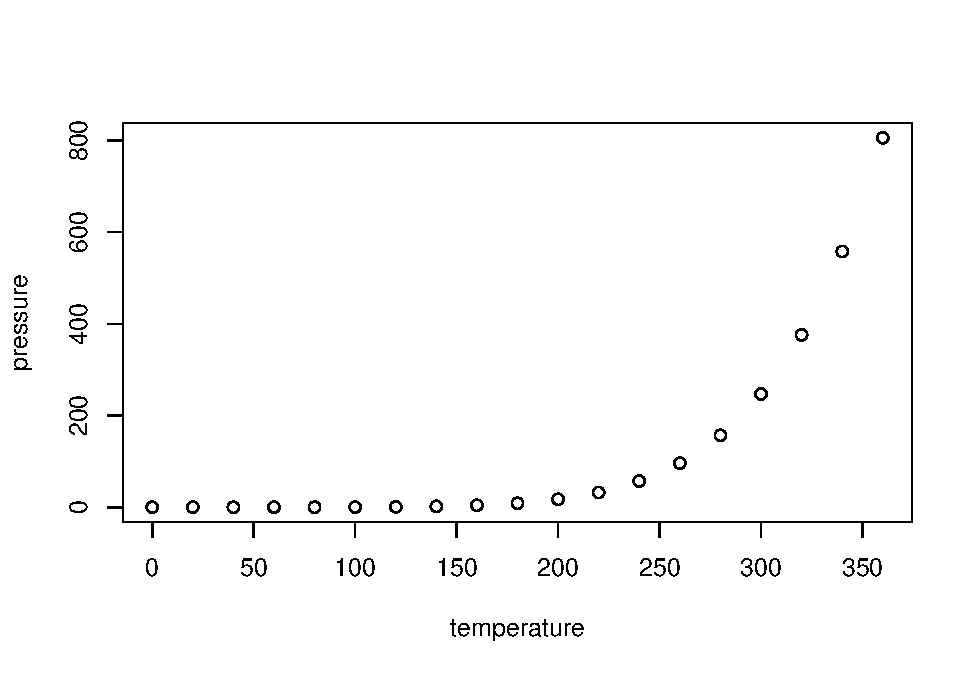
\includegraphics[width=0.8\linewidth]{MyBook_files/figure-latex/pressure-1} 

}

\caption{A figure}\label{fig:pressure}
\end{figure}

\normalsize

Figures can be created by the R code (figure \ref{fig:pressure}).
With Bookdown, a label is associated with each figure: its name is \texttt{fig:xxx} where \texttt{xxx} is the name of the R code snippet.
References are made with the command \texttt{\textbackslash{}@ref(fig:xxx)}.

The header of the code snippet of the figure \ref{fig:pressure} is:

\begin{verbatim}
```{r pressure, fig.cap="Title of the figure"}
```
\end{verbatim}

It contains at least the name of the figure and its caption.

The default width of figures is set in the option chunk in \texttt{index.Rmd}.
It is \texttt{out.width=\textquotesingle{}80\%\textquotesingle{}} in this template, i.e.~80\% of the width of the text.
If a full-width figure is needed, including the margin width, use \texttt{out.width=\textquotesingle{}\textbackslash{}\textbackslash{}widthw\textquotesingle{}} in its code chunk header.

When large margins are used in memoirs, figure captions are set in the margins of PDF outputs.
Margins can be used to enlarge a figure: add knitr options \texttt{out.width=\textquotesingle{}\textbackslash{}\textbackslash{}widthw\textquotesingle{}} and \texttt{fig.env=\textquotesingle{}figure\textquotesingle{}} in the code chunk header.
Figure alignment must be \texttt{fig.align\ =\ \textquotesingle{}center\textquotesingle{}} (which is by default).
The caption is then inserted below the figure.
Small figures can be put in the margin by the option \texttt{fig.env=\textquotesingle{}marginfigure\textquotesingle{}}.
These changes are ignored in the HTML output.

If the caption is long, the header is not easy to read.
Also, the caption is limited to simple text.
For more elaborate captions, it is possible to declare the caption in a separate paragraph that begins with the text \texttt{(ref:FigureName)}.
The figure \ref{fig:pressure2} benefits from an improved caption.



\scriptsize

\begin{figure}

{\centering 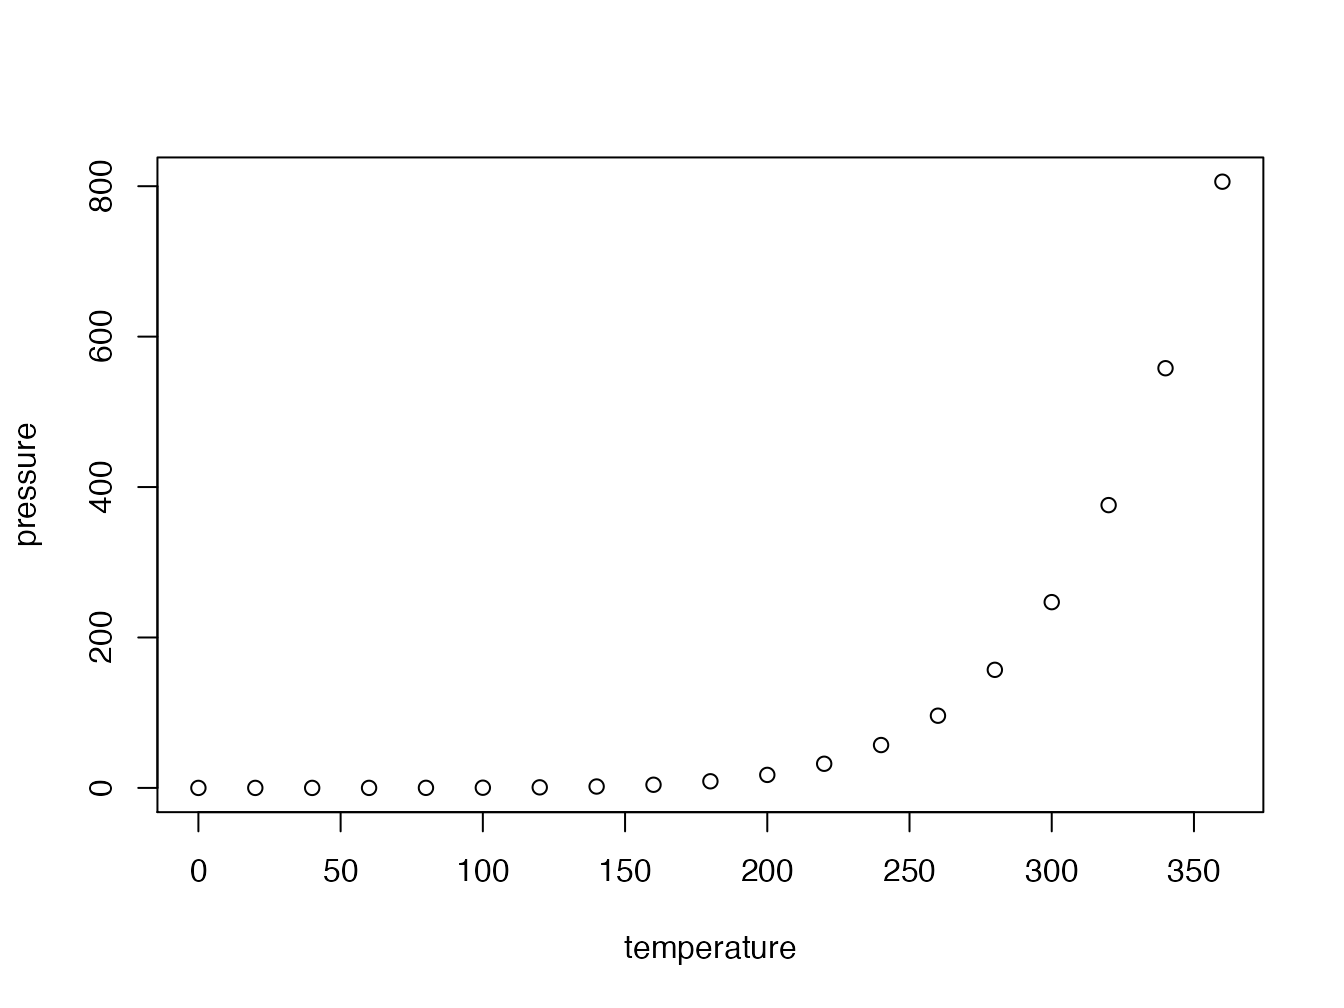
\includegraphics[width=0.8\linewidth]{MyBook_files/figure-latex/pressure2-1} 

}

\caption{Title with \emph{italic}, math (\(\sqrt\pi\)) and reference to figure \ref{fig:pressure}}\label{fig:pressure2}
\end{figure}

\normalsize

The text in \texttt{fig.cap}, ``Title of figure'' previously, is replaced by \texttt{(ref:pressure)} \emph{within the quotation marks} and the caption is entered in a paragraph starting with \texttt{(ref:pressure)} followed by a space.
Captions are limited to a single paragraph.
They should not contain bibliographic references or references to the figures may not find them: if necessary, cite the source of a figure in the text.

Figures that are not created by R but come from files are embedded in a piece of code by the \texttt{include\_graphics()} function whose argument is the file containing the image to be displayed.
Always place these files in the \texttt{images} folder for good organization.

\hypertarget{tables}{%
\section{Tables}\label{tables}}

The horizontal - and vertical separators \textbar{} allow to draw a table according to the Markdown syntax, but it is not the best method.

Tables can also be produced by R code.
The content of the table is in a dataframe.
The \texttt{kable} function in the \emph{knitr} package prepares the table for display and passes the result to the \texttt{kable\_styling} function in the \emph{kableExtra} package for final formatting.

\scriptsize

\begin{Shaded}
\begin{Highlighting}[]
\FunctionTok{library}\NormalTok{(}\StringTok{"tidyverse"}\NormalTok{)}
\FunctionTok{names}\NormalTok{(iris) }\OtherTok{\textless{}{-}} \FunctionTok{c}\NormalTok{(}\StringTok{"Sepal length ($l\_s$)"}\NormalTok{, }\StringTok{"Width"}\NormalTok{, }\StringTok{"Petal length"}\NormalTok{,}
    \StringTok{"Width"}\NormalTok{, }\StringTok{"Species"}\NormalTok{)}
\NormalTok{knitr}\SpecialCharTok{::}\FunctionTok{kable}\NormalTok{(}\FunctionTok{head}\NormalTok{(iris), }\AttributeTok{caption =} \StringTok{"Table created by R"}\NormalTok{, }\AttributeTok{booktabs =} \ConstantTok{TRUE}\NormalTok{,}
    \AttributeTok{escape =} \ConstantTok{FALSE}\NormalTok{) }\SpecialCharTok{\%\textgreater{}\%}
\NormalTok{    kableExtra}\SpecialCharTok{::}\FunctionTok{kable\_styling}\NormalTok{(}\AttributeTok{bootstrap\_options =} \StringTok{"striped"}\NormalTok{,}
        \AttributeTok{full\_width =} \ConstantTok{FALSE}\NormalTok{)}
\end{Highlighting}
\end{Shaded}

\begin{table}

\caption{\label{tab:kable}Table created by R}
\centering
\begin{tabular}[t]{rrrrl}
\toprule
Sepal length ($l_s$) & Width & Petal length & Width & Species\\
\midrule
5.1 & 3.5 & 1.4 & 0.2 & setosa\\
4.9 & 3.0 & 1.4 & 0.2 & setosa\\
4.7 & 3.2 & 1.3 & 0.2 & setosa\\
4.6 & 3.1 & 1.5 & 0.2 & setosa\\
5.0 & 3.6 & 1.4 & 0.2 & setosa\\
\addlinespace
5.4 & 3.9 & 1.7 & 0.4 & setosa\\
\bottomrule
\end{tabular}
\end{table}

\normalsize

The caption is specified by the \texttt{caption} argument and referencing is possible because the table is given a label whose name is \texttt{tab:} followed by the name of the code snippet (table \ref{tab:kable}).
As with figures, an enhanced legend can be written in a separate paragraph.

Always use the \texttt{booktabs\ =\ TRUE} argument so that the thickness of the separator lines is optimal in LaTeX.
Since the table contains mathematics (in the name of the first column), the \texttt{escape\ =\ FALSE} option is necessary.

The \texttt{bootstrap\_options\ =\ "striped"} style option provides more readable tables in HTML.
Last, the \texttt{full\_width\ =\ FALSE} option allows you to adjust the width of the table to its content instead of occupying all the available width.

\hypertarget{maths}{%
\section{Maths}\label{maths}}

Equations in LaTeX format can be inserted in line, like \(A=\pi r^2\) (code: \texttt{\$A=\textbackslash{}pi\ r\^{}2\$}) or isolated (the \$ are doubled) like \[e^{i \pi} = -1.\]

They can be numbered: see equation \eqref{eq:disk}, using the \texttt{\textbackslash{}equation} environment.

\begin{equation}
  A = \pi r^2.
  \label{eq:disk}
\end{equation}

The numbered equation is created by the following code:

\begin{verbatim}
\begin{equation}
  A = \pi r^2.
  \label{eq:disk}
\end{equation}
\end{verbatim}

\hypertarget{cross-references}{%
\section{Cross-references}\label{cross-references}}

Figures and tables have an automatically generated label, identical to the name of the code snippet prefixed with \texttt{fig:} and \texttt{tab:}.

For equations, the label is added manually by the code \texttt{(\textbackslash{}\#eq:xxx)} before the end of the equation.

Sections can be tagged by ending their title with \texttt{\{\#yyy\}}.

In all cases, the call to the reference is made by the command \texttt{\textbackslash{}@ref()}.

\hypertarget{bibliography}{%
\section{Bibliography}\label{bibliography}}

Bibliographic references in bibtex format must be included in the \texttt{.bib} file declared in the header of the Markdown document.

\begin{verbatim}
bibliography: references.bib
\end{verbatim}

They can be called in the text, between brackets by the code \texttt{{[}@CitationKey{]}}, as sidenotes \autocite{Xie2016}, or without square brackets, to include the authors' names in the text, such as \textcite{Xie2018} .

Bibliography is handled by pandoc when producing Word or HTML documents.
The bibliographic style can be specified, by adding the line

\begin{verbatim}
csl:file_name.csl
\end{verbatim}

in the document header and copying the \emph{.csl} style file into the project folder.
The default style (if no csl is specified) is ``chicago-author-date''.
Several thousand styles are available \footnote{\url{https://github.com/citation-style-language/styles}}.

For PDF documents, the bibliography is handled by BibLaTeX, see section \ref{index}.

\hypertarget{forcing-line-breaks}{%
\section{Forcing line breaks}\label{forcing-line-breaks}}

Hyphenation is handled automatically in LaTeX.
If a word is not hyphenated correctly, add its hyphenation in the preamble of the file with the command \texttt{hyphenation} (words are separated by spaces, hyphenation locations are represented by dashes).

If LaTeX can't find a solution for the line break, for example because some code is too long a non-breaking block, add the LaTeX command \texttt{\textbackslash{}break} to the line break location.
Do not leave a space before the command.
The HTML document ignores LaTeX commands.

\hypertarget{sec:languages}{%
\section{Languages}\label{sec:languages}}

Languages are declared in the document header.

The main language of the document (\texttt{lang}) changes the name of some elements, such as the table of contents.
The change of language in the document (one of \texttt{otherlangs}) is managed in LaTeX but not in HTML by inserting on a new line the following command:

\begin{verbatim}
\selectlanguage{english}
\end{verbatim}

The current language has an effect only in LaTeX output: a space is added before double punctuation in French, the size of spaces is larger at the beginning of sentences in English, etc.
The \texttt{\textbackslash{}selectlanguage} command is simply ignored in HTML.

Language codes are used in the header, such as \texttt{en-US} but language names are necessary in \texttt{\textbackslash{}selectlanguage\{\}}.
Name matches are listed in table 3 of the polyglossia package documentation\footnote{\url{http://mirrors.ctan.org/macros/unicodetex/latex/polyglossia/polyglossia.pdf}}.

\hypertarget{chapter-summary}{%
\section{Chapter summary}\label{chapter-summary}}

The take-home message of each chapter can be displayed in a box, see the beginning of this one.
The code is that of a code block of type ``Summary''.

\begin{verbatim}
```{block, type='Summary'}
Some text for this block.
```
\end{verbatim}

Its heading text is set in the header of \texttt{index.Rmd}:

\begin{verbatim}
chaptersummary: In a Nutshell
\end{verbatim}

\hypertarget{documentation}{%
\section{Documentation}\label{documentation}}

\hypertarget{user-documentation}{%
\subsection{User documentation}\label{user-documentation}}

\begin{itemize}
\tightlist
\item
  The book \href{https://bookdown.org/yihui/bookdown/}{bookdown: Authoring Books and Technical Documents with R Markdown} by Yihui Xie, the author of \textbf{bookdown} and \textbf{knitr}.
  All the necessary details for writing (writing equations, cross-references, etc.) are given.
\item
  The \href{https://www.rstudio.com/wp-content/uploads/2015/02/rmarkdown-cheatsheet.pdf}{R Markdown cheat sheet} for the syntax.
\end{itemize}

\hypertarget{documentation-for-developers}{%
\subsection{Documentation for developers}\label{documentation-for-developers}}

\begin{itemize}
\tightlist
\item
  \href{http://rmarkdown.rstudio.com/pdf_document_format.html\#advanced_customization}{LaTeX file format customization}.
\item
  The \href{https://pandoc.org/MANUAL.html}{Pandoc manual} for possible options in the YAML header.
\end{itemize}


% Bibliography
%%%%%%%%%%%%%%%%%%%%%%%%%%%%%%%%%%%%%%%%%%%%%%%%%%%%%%%%%%

\backmatter
\SmallMargins

\printbibliography
\onecolumn


% Tables (of tables, of figures)
%%%%%%%%%%%%%%%%%%%%%%%%%%%%%%%%%%%%%%%%%%%%%%%%%%%%%%%%%%


\cleardoublepage
\LargeMargins
\listoffigures


% After-body (LaTeX code inclusion)
%%%%%%%%%%%%%%%%%%%%%%%%%%%%%%%%%%%%%%%%%%%%%%%%%%%%%%%%%%




% Back cover
%%%%%%%%%%%%%%%%%%%%%%%%%%%%%%%%%%%%%%%%%%%%%%%%%%%%%%%%%%%

% Even page, small margins, no running head, no page number.
\evenpage
\SmallMargins
\thispagestyle{empty}

\begin{normalsize}

\begin{description}

\selectlanguage{english}
\item[Abstract]
English abstract, on the last page.

This is a bookdown template based on LaTeX memoir class.
\item[Keywords]
Keyword in English, As a list.
~\\

\end{description}

\end{normalsize}

\vspace*{\fill}
\centering
\includegraphics[width=.3\textwidth]{images/logo}

\end{document}
